\documentclass[aspectratio=169]{beamer}
\usepackage{lmodern}
\usetheme{Madrid}
%\usecolortheme{giantoak}
\newcommand*\oldmacro{}
\let\oldmacro\insertshorttitle
\renewcommand*\insertshorttitle{\oldmacro\hfill\insertframenumber\,/\,\inserttotalframenumber}
\usepackage[framemethod=tikz]{mdframed}

\usepackage{beamerthemesplit}
\usepackage{textpos}
\usepackage{pgf}
%\logo{\pgfputat{\pgfxy(0,-.4)}{\pgfbox[right,base]{\includegraphics[height=1.0cm]{logo.jpg}}}}
%\newcommand{\nologo}{\setbeamertemplate{logo}{}}
\usepackage{booktabs}
\usepackage{graphicx}
\theoremstyle{principle}
\newtheorem*{principle}{Design Principle}


\titlegraphic{\includegraphics[width=1.0\paperwidth]{cool-wind-800px.jpg}}

\title{Amendments}
%\author[Jeremy Kedziora]{Wind Data Science Team\\
%\small{Uptake}}
\date{}

\begin{document}

%{
%%\nologo
%\begin{frame}
%    \maketitle
%\end{frame}
%}
%pages 1-7, 8-9, 14-15.


{
  \usebackgroundtemplate{\includegraphics[width=1.0\paperwidth]{GI_bill_signing.jpg}}
  \begin{frame}[plain]
  
\begin{mdframed}[tikzsetting={draw=black,fill=white,fill opacity=0.7,
               line width=0pt},backgroundcolor=none,leftmargin=20,
               rightmargin=20,innertopmargin=4pt]
\Huge A Case Study in Policy Evaluation
\end{mdframed}

  \end{frame}
}

%@@@@@@@@@@@@@@@@@@@@@@@@@@@@@@@@@@@@@@@@@@@@@@@@@
%\begin{frame}
%
%\begin{center}
%
\includegraphics[scale=0.4]{lake_michigan.jpg}
%\end{center}
%
%
%\end{frame}

%@@@@@@@@@@@@@@@@@@@@@@@@@@@@@@@@@@@@@@@@@@@@@@@@@
\begin{frame}
    \begin{center}
     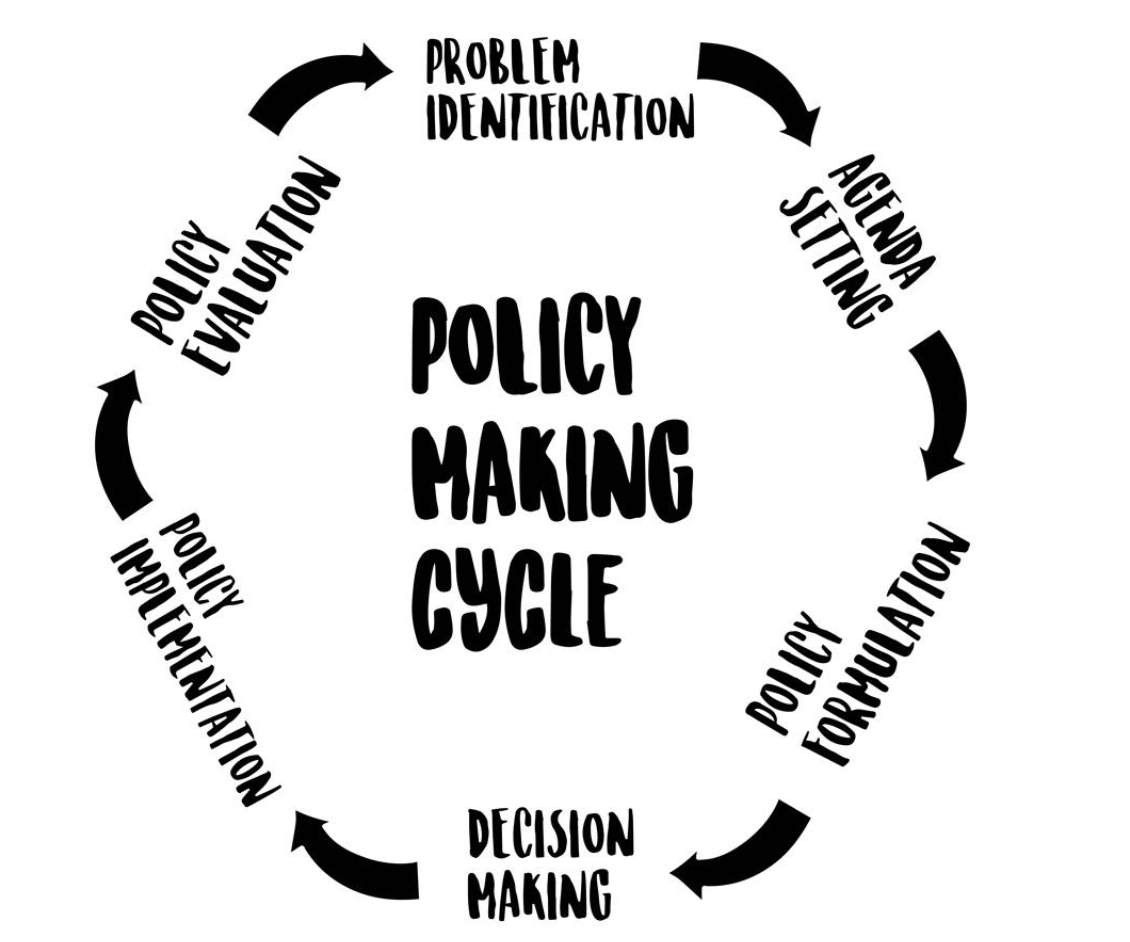
\includegraphics[scale=0.4]{policy_process.png}
     \end{center}
\end{frame}

%@@@@@@@@@@@@@@@@@@@@@@@@@@@@@@@@@@@@@@@@@@@@@@@@@
\begin{frame}
\frametitle{Birkland$+$ Model of Policy, goals, problems}
\begin{itemize}
\item Policy Domain: what substantive problems are under consideration?  This specifies:
\begin{itemize}
\item The actors involved, official actors who can make decisions $+$ \textbf{stakeholders}; 
\item \textbf{Distribution of benefits/costs} $\Rightarrow$ actor organization, e.g. iron triangle, policy community;
\item The systemic agenda; 
\end{itemize}
\bigskip
\item \color{black}Input-output Model;
\begin{itemize}
\item Actors: \textbf{legislature, executive, bureaucrats, justices and the available levers};
\item Inputs: \textbf{agenda setting (application of power/social construction, focusing events, indicator change driven esp by unofficial actors)} \textbf{sets goals}, \textbf{determines the causal model}, which specifies the institutional agenda, and leads to the \textbf{policies} on the decision agenda;
\item Black box \textbf{decision making, timing (incrementalism, punctuated eq) driven by indicators/focusing events}, choice driven by e.g. median voter thm, Arrow's thm;
\begin{itemize}
\item Round 1: \textbf{works on decision agenda}, leads to outputs (e.g. statute laws, rules, court decisions);
\item Round 2: \textbf{Implementation}, leads to outcomes;
 \end{itemize}
\end{itemize}
\bigskip
\item Outcomes: \textbf{Feedback from failure and success}, learning leads to iteration and updates.
\end{itemize}
\end{frame}

%@@@@@@@@@@@@@@@@@@@@@@@@@@@@@@@@@@@@@@@@@@@@@@@@@
\begin{frame}
\frametitle{Learning}

\begin{itemize}
\item Single loop learning: optimizing and adjusting policy;
\bigskip
\item Double loop learning: optimizing/adjusting fundamental values/logic that leads to policy;
\bigskip
\item Instrumental policy learning: effectiveness of policy tools;
\bigskip
\item Social policy learning: causes of problems;
\bigskip
\item Political learning: better arguments in policy debates.
\end{itemize}

\end{frame}

%@@@@@@@@@@@@@@@@@@@@@@@@@@@@@@@@@@@@@@@@@@@@@@@@@
\begin{frame}
\frametitle{Purpose of the paper:}
\begin{itemize}
\item The GI bill (i.e. Servicemen's Readjustment Act of 1944) was a large scale social entitlement program funded by federal government:
\begin{itemize}
\item Access to higher education;
\item Access to vocational training;
\item Unemployment benefits (20/52);
\item Access to home ownership (low interest no downpayment mortgages);
\end{itemize}
\bigskip
\bigskip
\item 51\% of all returning veterans -- about 7.8 million people -- took advantage of it;
\begin{itemize}
\item 2.2 million college attendees;
\item 5.6 million vocational/on-the-job training;
\end{itemize}
\bigskip
\bigskip
\item Mettler's question: \textbf{did it work}? Does it:
\begin{itemize}
\item promote citizen involvement in democracy (e.g. give something back effect or incorporation)?
\item discourage citizen involvement in democracy (e.g. we've got what we need to we're out)?
\item generate only social and economic effects?
\end{itemize}
\end{itemize}
\end{frame}

%@@@@@@@@@@@@@@@@@@@@@@@@@@@@@@@@@@@@@@@@@@@@@@@@@
\begin{frame}
\frametitle{What is policy feedback?}
\begin{itemize}
\item \textbf{Policy feedback} is a theoretical idea -- that policies can change political participation which can then change policy-making;
\bigskip
\bigskip
\item So what evidence is there for these sorts of feedback effects?
\begin{itemize}
\item Farmers vote at higher rates (Wolfinger and Rosenstone 1980);
\item SS/medicare beneficiaries get involved at higher rates (Rosenstone and Hansen 1993);
\end{itemize}
\bigskip
\bigskip
\item What mechanisms explain variation in effects?
\begin{itemize}
\item Program clients learn from the particular program they interact with $\Rightarrow$ distinct rules create distinct effects (Soss 1999);
\item Client background varies systematically with program (Campbell 2000).
\end{itemize}
\end{itemize}
\end{frame}

%@@@@@@@@@@@@@@@@@@@@@@@@@@@@@@@@@@@@@@@@@@@@@@@@@
\begin{frame}
\frametitle{Mettler's Theory}

\begin{center}
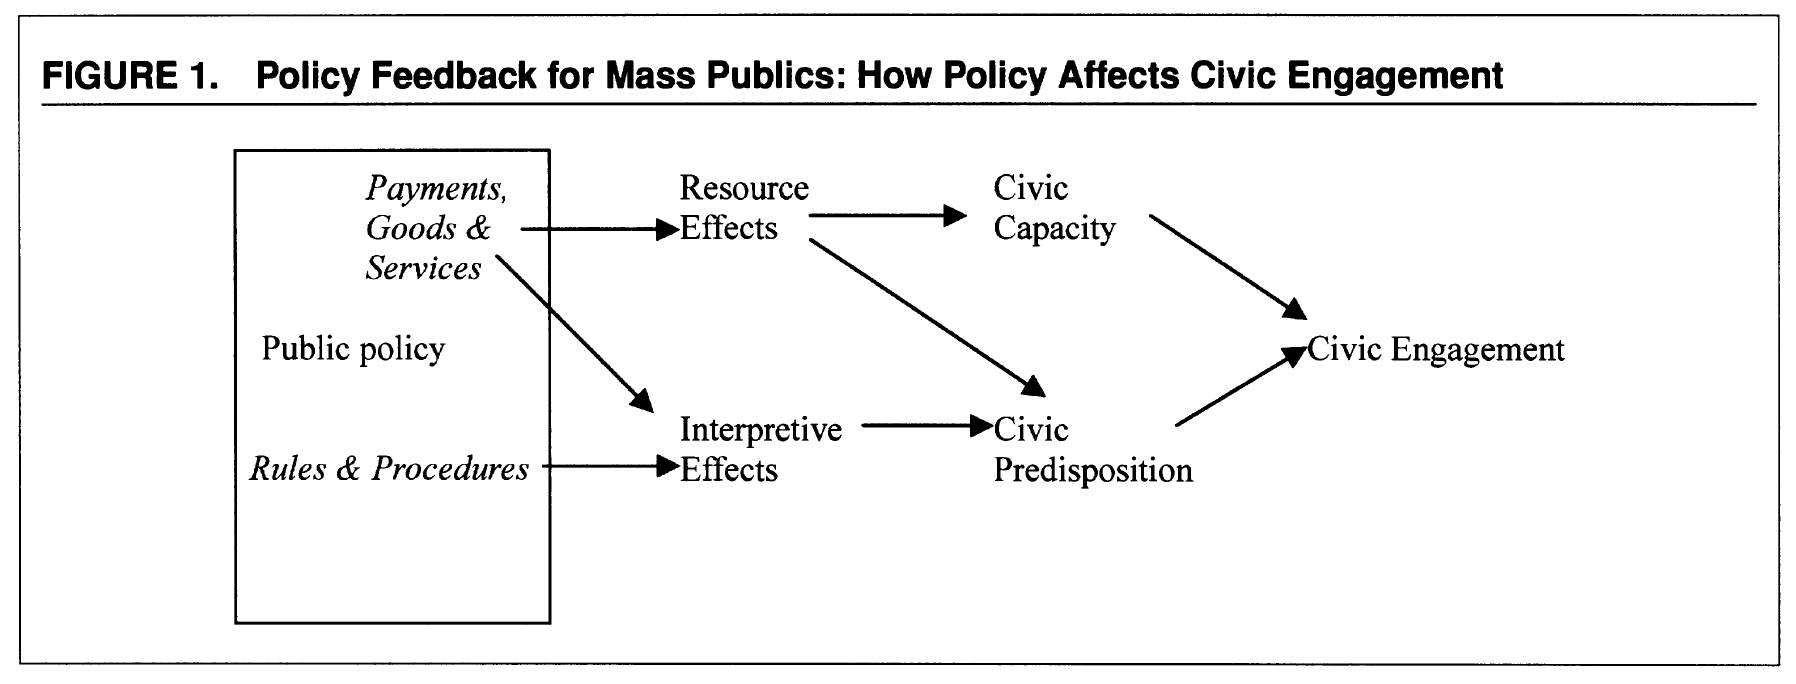
\includegraphics[scale=0.45]{Mettlers_theory.png}
\end{center}

\end{frame}

%@@@@@@@@@@@@@@@@@@@@@@@@@@@@@@@@@@@@@@@@@@@@@@@@@
\begin{frame}
\frametitle{Testing the model}
\begin{itemize}
\item Hypotheses from existing theories about GI bill:
\begin{itemize}
\item \textbf{Preexisting characteristics} -- omitted variables, other things cause both participation and program use;
\item \textbf{By-product explanation} -- policy design is irrelevant, education promotes participation;
\item \textbf{Passivity explanation} -- beneficiaries exhibit lower levels of involvement in public life than those who did not rely on government benefits to fund their education;
\end{itemize}
\bigskip
\bigskip
\item Mettler's policy feedback model: GI bill had resource and incentive effects that increased participation:
\begin{itemize}
\item \textbf{Reciprocity explanation} -- a sense of giving back, e.g. in comparison to WWI vets;
\item \textbf{Critical effects explanation} -- G.I. Bill incorporated less advantaged citizens more fully;
\end{itemize}
\bigskip
\bigskip
\item Research design:
\begin{itemize}
\item Mail survey to 1000 vets (four units, two Army and two Air Force) including questions on participation, military service, GI bill use, occupation, demographics;
\item Dependent variable: civic group membership (e.g. Lions clubs, PTA), political participation (e.g. campaign work, contributions).
\end{itemize}
\end{itemize}
\end{frame}

%@@@@@@@@@@@@@@@@@@@@@@@@@@@@@@@@@@@@@@@@@@@@@@@@@
\begin{frame}
\frametitle{Testing the model: results}
\begin{columns}
\begin{column}{0.5\textwidth}
\begin{itemize}
\item Participation $\neq$ SEC $\Rightarrow$ Preexisting characteristics insufficient;
\bigskip
\item Participation $\neq$ Education $\Rightarrow$ by-product insufficient;
\bigskip
\item Effect of GI bill positive $\Rightarrow$ passivity insufficient;
\end{itemize}
\end{column}
\begin{column}{0.5\textwidth}
\begin{center}
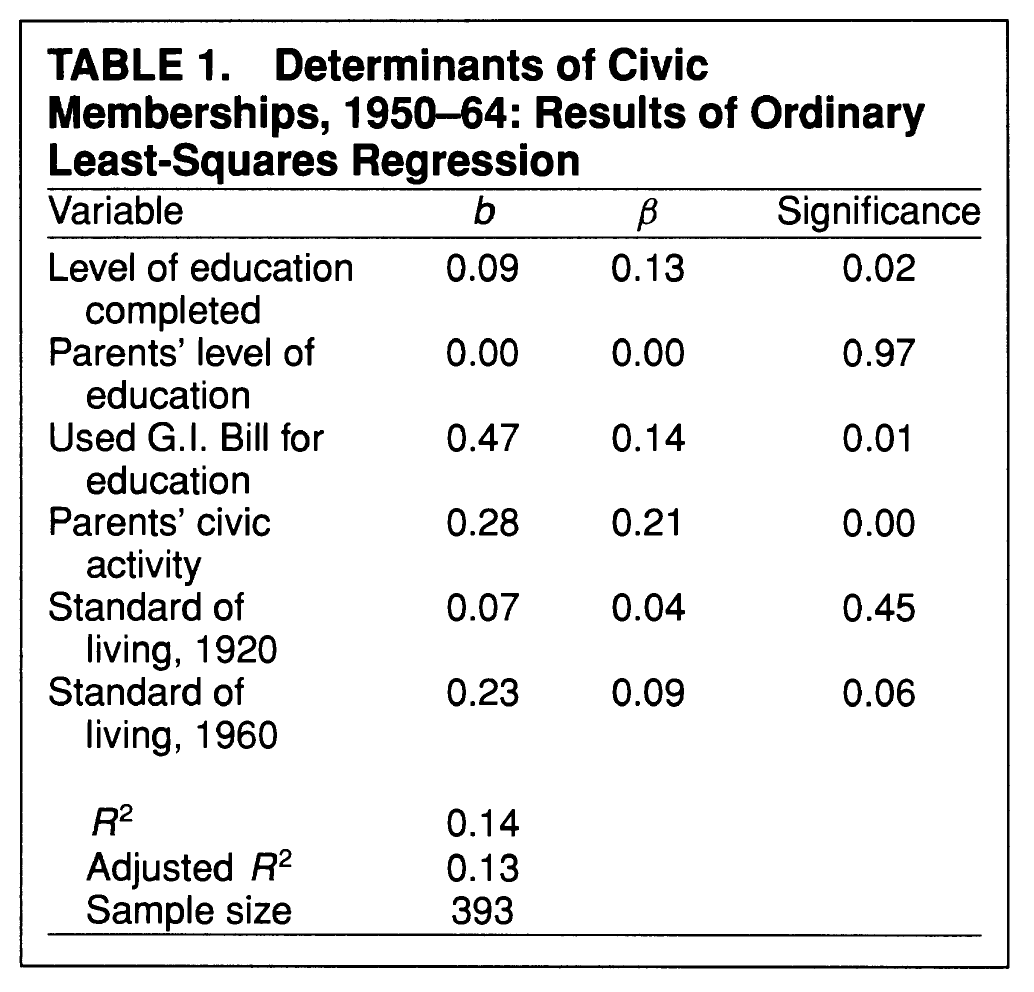
\includegraphics[scale=0.4]{table_1.png}
\end{center}
\end{column}
\end{columns}
\end{frame}

%@@@@@@@@@@@@@@@@@@@@@@@@@@@@@@@@@@@@@@@@@@@@@@@@@
\begin{frame}
\frametitle{Testing the model: results}
\begin{columns}
\begin{column}{0.5\textwidth}
\begin{itemize}
\item Participation $\neq$ SEC $\Rightarrow$ Preexisting characteristics insufficient;
\bigskip
\item Participation $\neq$ Education $\Rightarrow$ by-product insufficient;
\bigskip
\item Effect of GI bill positive $\Rightarrow$ passivity insufficient;
\end{itemize}
\end{column}
\begin{column}{0.5\textwidth}
\begin{center}
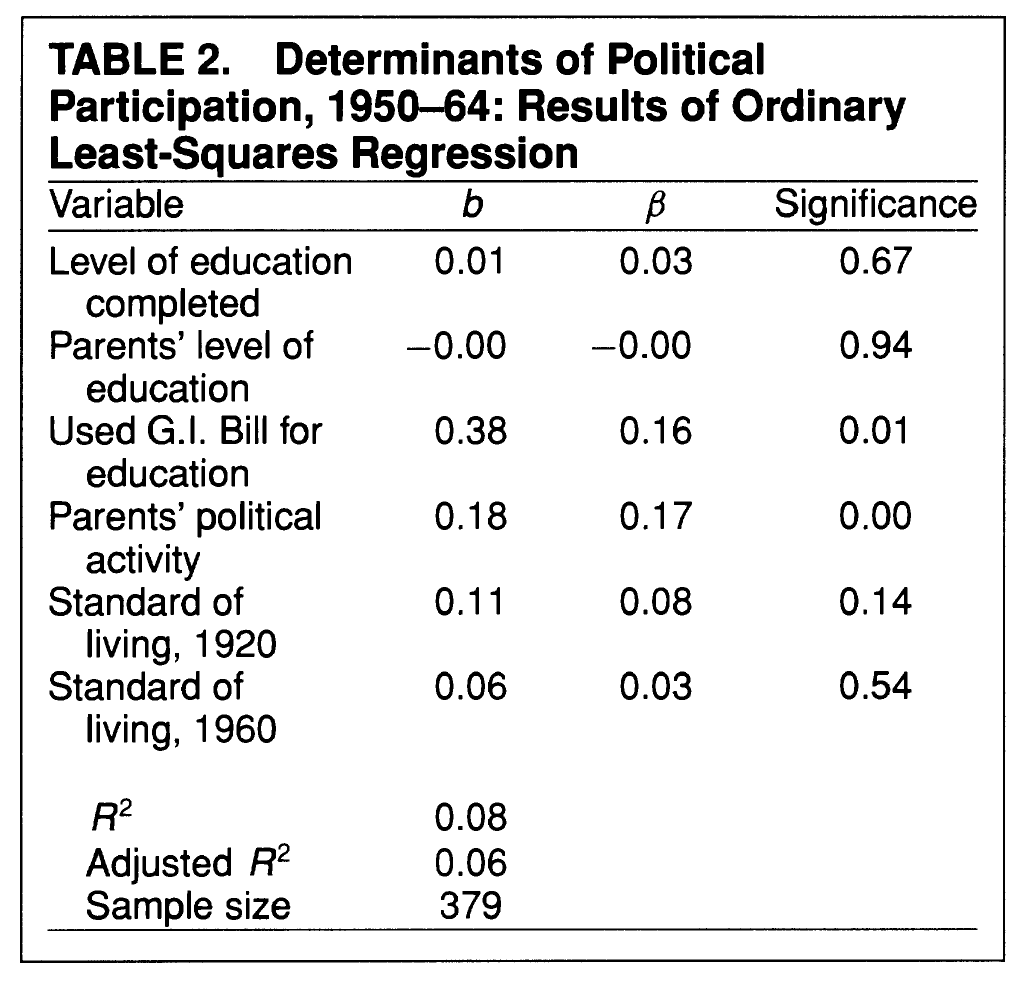
\includegraphics[scale=0.4]{table_2.png}
\end{center}
\end{column}
\end{columns}
\end{frame}

%@@@@@@@@@@@@@@@@@@@@@@@@@@@@@@@@@@@@@@@@@@@@@@@@@
\begin{frame}
\frametitle{Testing the model: reciprocity vs critical effects}
\begin{columns}
\begin{column}{0.5\textwidth}

\begin{itemize}
\item Nearly all respondents viewed military service as civic obligation and therefore GI bill as a privilege not a right;
\bigskip
\bigskip
\item Respondents did not view GI bill use as obligating them to give back in a transactional sense;
\bigskip
\bigskip
\item Results suggest reciprocity an explanation for civic membership but not political participation.
\end{itemize}
\end{column}
\begin{column}{0.5\textwidth}
\begin{center}
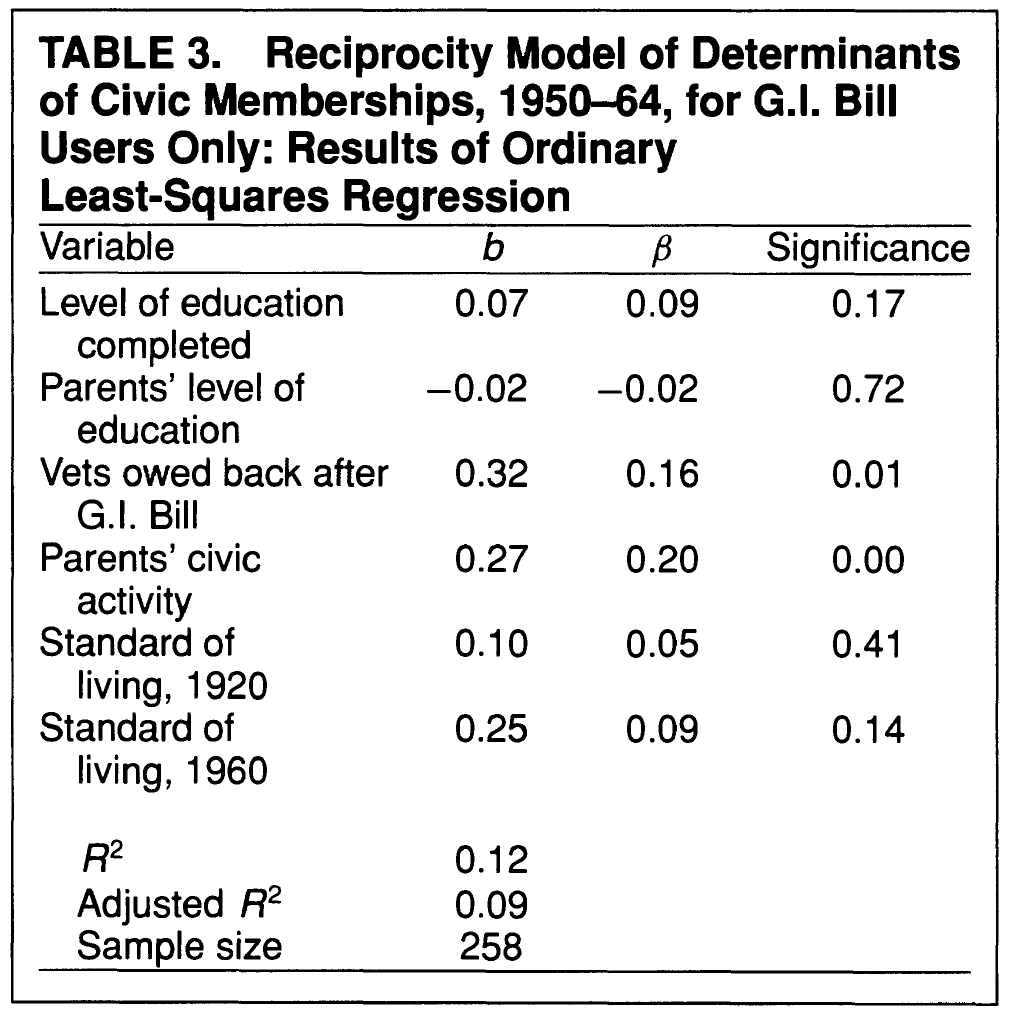
\includegraphics[scale=0.4]{table_3.png}
\end{center}
\end{column}
\end{columns}

\end{frame}

%@@@@@@@@@@@@@@@@@@@@@@@@@@@@@@@@@@@@@@@@@@@@@@@@@
\begin{frame}
\frametitle{Testing the model: reciprocity}
\begin{columns}
\begin{column}{0.5\textwidth}

\begin{itemize}
\item Nearly all respondents viewed military service as civic obligation and therefore GI bill as a privilege not a right;
\bigskip
\bigskip
\item Respondents did not view GI bill use as obligating them to give back in a transactional sense;
\bigskip
\bigskip
\item Results suggest reciprocity an explanation for civic membership but not political participation.
\end{itemize}
\end{column}
\begin{column}{0.5\textwidth}
\begin{center}
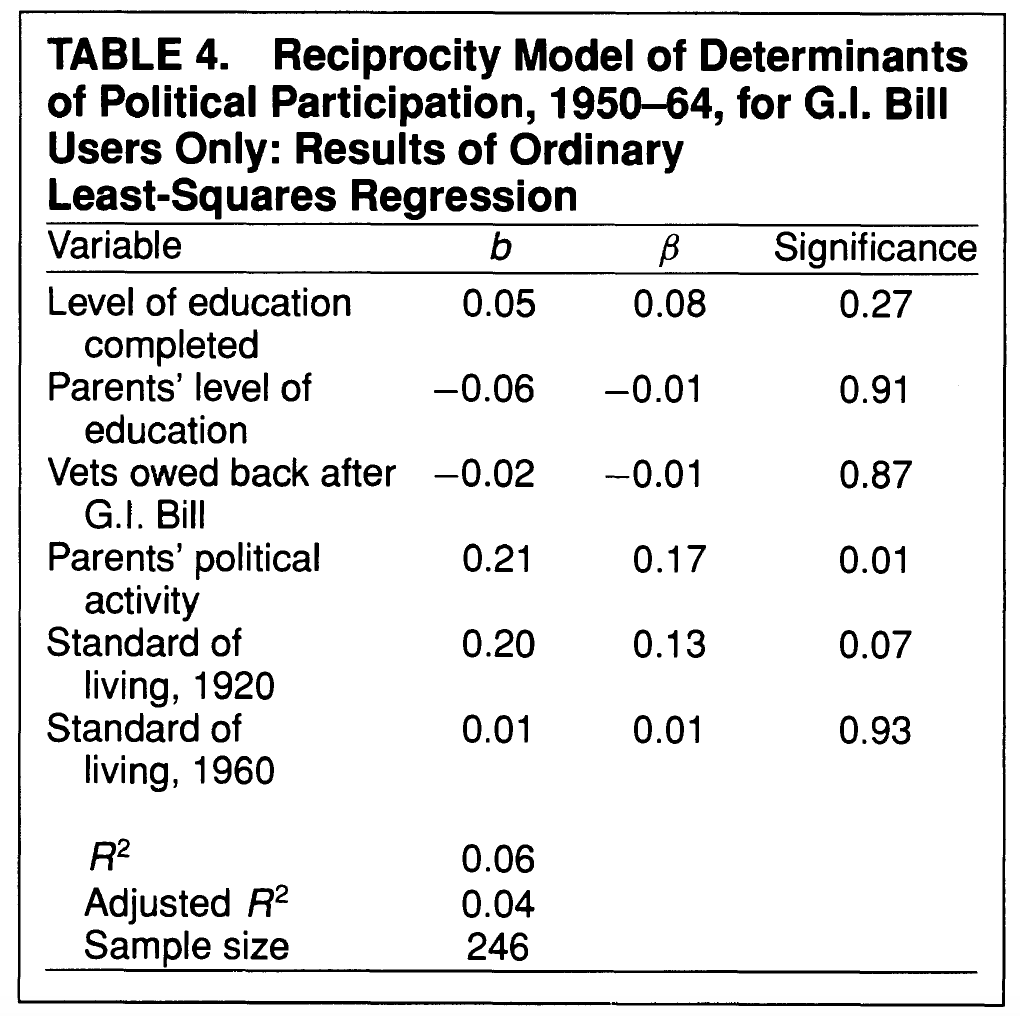
\includegraphics[scale=0.4]{table_4.png}
\end{center}
\end{column}
\end{columns}

\end{frame}

%@@@@@@@@@@@@@@@@@@@@@@@@@@@@@@@@@@@@@@@@@@@@@@@@@
\begin{frame}
\frametitle{Testing the model: critical effects}
\begin{columns}
\begin{column}{0.5\textwidth}

\begin{itemize}
\item Targeted resource effects: educational benefits were most consequential for those from low/moderate SEC (Yes);
\bigskip
\bigskip
\item Targeted interpretive effects: bestowing dignity via equal treatment (Yes);
\bigskip
\bigskip
\item Mettler: sign/sig on interaction term $\Rightarrow$ critical effects increased participation.
\end{itemize}
\end{column}
\begin{column}{0.5\textwidth}
\begin{center}
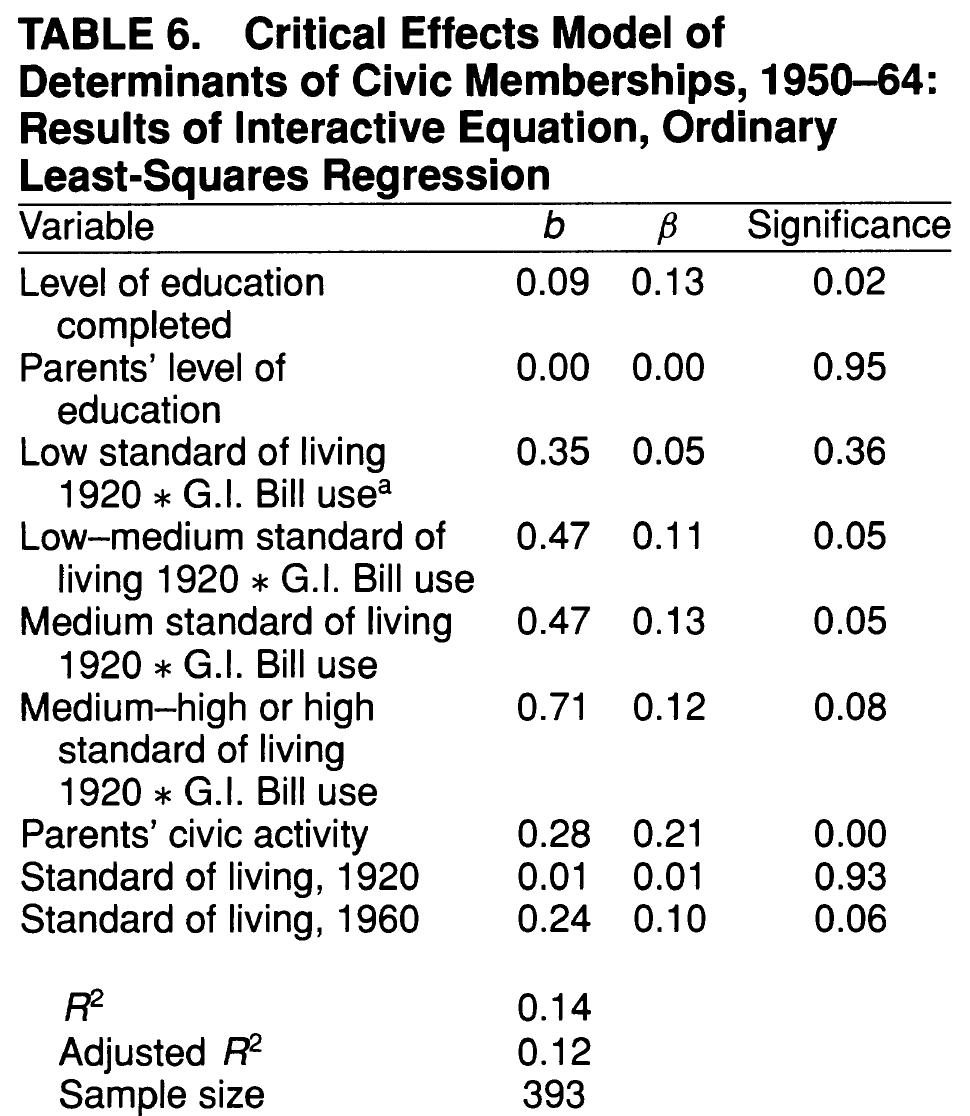
\includegraphics[scale=0.35]{table_6.png}
\end{center}
\end{column}
\end{columns}

\end{frame}

%@@@@@@@@@@@@@@@@@@@@@@@@@@@@@@@@@@@@@@@@@@@@@@@@@
\begin{frame}
\frametitle{Testing the model: critical effects}
\begin{columns}
\begin{column}{0.5\textwidth}

\begin{itemize}
\item Targeted resource effects: educational benefits were most consequential for those from low/moderate SEC (Yes);
\bigskip
\bigskip
\item Targeted interpretive effects: bestowing dignity via equal treatment (Yes);
\bigskip
\bigskip
\item Mettler: sign/sig on interaction term $\Rightarrow$ critical effects increased participation.
\end{itemize}
\end{column}
\begin{column}{0.5\textwidth}
\begin{center}
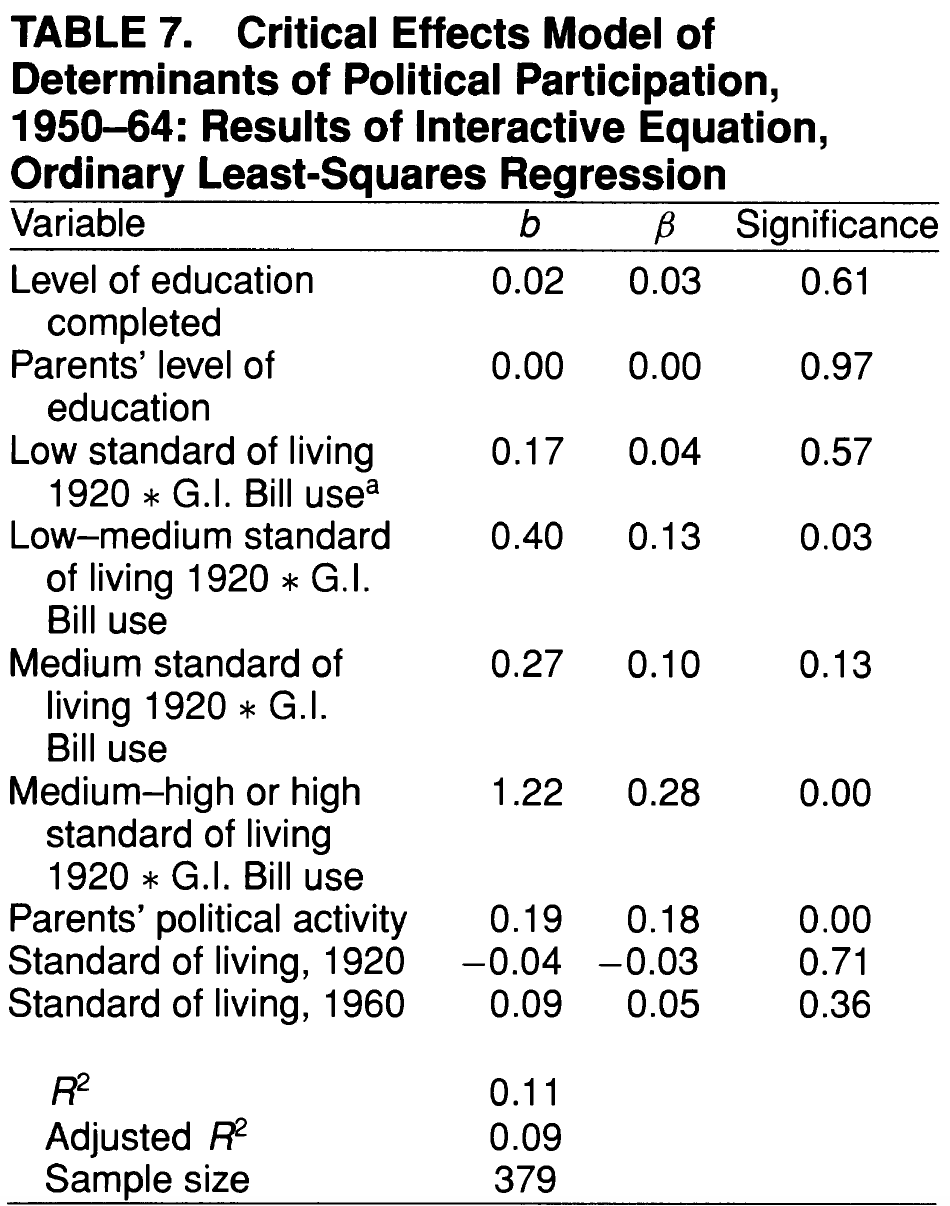
\includegraphics[scale=0.35]{table_7.png}
\end{center}
\end{column}
\end{columns}

\end{frame}

%@@@@@@@@@@@@@@@@@@@@@@@@@@@@@@@@@@@@@@@@@@@@@@@@@
\begin{frame}
\frametitle{Conclusion}
\begin{quote}
The case of the G.I. Bill illustrates how a public policy can function, like any institution, in promoting norms; in this case, it fostered participatory norms and the development of social capital. In contrast to most determinants of participation, the G.I. Bill promoted civic participation among groups that were somewhat less advantaged in the typical prerequisites for participation. As beneficiaries became more fully incorporated through social rights, they responded through more active forms of participatory citizenship.
\end{quote}

\end{frame}

%@@@@@@@@@@@@@@@@@@@@@@@@@@@@@@@@@@@@@@@@@@@@@@@@@
\begin{frame}
\frametitle{Some Critiques...}
\begin{itemize}

\item Sampled units/time means only certain types enter the sample, e.g. segregation/age:
\begin{itemize}
\item Excluded populations correlated with GI Bill use and civic engagement $\Rightarrow$ estimates are wrong;
\item Example: older people less likely to use GI Bill and more likely to participate in civic engagement $\Rightarrow$ overestimate of GI Bill effect;
\end{itemize}
\bigskip
\item Differential death rates:
\begin{itemize} 
\item GI Bill users are overrepresented in sample;
\item Example: wealth improves lifespan, friendships (civic engagement) improve lifespan, so you might undersample poor, nonengaged people $\Rightarrow$ underestimate of GI bill effect;
\end{itemize}
\bigskip
\item Time slice effect of GI bill:
\begin{itemize}
\item Participation in civic groups at all time high immediately post WWII; 
\item Effect of GI Bill on civic participation might look very different depending on time period.
\end{itemize}

\end{itemize}

\end{frame}

%@@@@@@@@@@@@@@@@@@@@@@@@@@@@@@@@@@@@@@@@@@@@@@@@@
\begin{frame}
\frametitle{More Critiques...}
\begin{itemize}
\item Choice of variables to include is arbitrary -- $\geq$ 64 models possible for Table 1;
\bigskip
\item Endogeneity -- what if participation causes one or more of the explanatory variables?  e.g. civic engagement or political activity could cause changes in 1960 standard of living $\Rightarrow$ estimate of variable effects will be wrong;
\bigskip
\item Model functional form misspecification (e.g. regression instead of a count model);
\bigskip
\item Omitted Variables -- e.g. civic memberships as an explanatory variable for table 2.

\end{itemize}
\end{frame}

\end{document}






